\documentclass[wide]{adonis}
\usepackage{hyperref}
\usepackage{tabularx}
\usepackage{xurl}
\usepackage{graphicx}

% more elegant citation without brackets
\makeatletter
%\def\@biblabel#1{}
\renewcommand\@cite[2]{{#1\if@tempswa,\nolinebreak[3] #2\fi}}
\makeatother

% main details
\title{Artificial Democracy}
\subtitle{Essay by}
\author{Richard Ebock}

% secondary details
\version{\today}

% headers
\runningauthor{Richard Ebock}
\runningtitle{Artificial Democracy}


\begin{document}
	\maketitle	
        
        %introduction section
	\section{Introduction}
            The year 2024 will be the most significant electoral year in history, with up to half of humanity having the opportunity to participate in votes. Over the year, new representatives of political institutions will be elected in Russia, India, South Africa, the European Union, the United States of America, and other regions.\\
            Free elections are a defining characteristic of democracy, giving citizens a voice to represent their individual interests. They determine the trajectory of a state's domestic and foreign policies for the upcoming term and have consequently been subject to internal and external manipulation for decades. In this pursuit, state-of-the-art technology has consistently played a decisive role. In particular, the recent advances in the field of \textit{Artificial Intelligence (AI)} and new associated technologies, such as \textit{deepfakes}, will have a profound impact on how voters make their decisions. \\
            As a computer scientist by training, subjects like Artificial Intelligence or \textit{Machine Learning} do not only make up a significant part of my academic curriculum, but are also at the very top of research and work opportunities. However, most importantly, my field of studies grants me insights into the working principles of these potent technologies.\\
            With this essay, I intend to move beyond the scope of mathematics and instead adopt an interdisciplinary approach, arguing that Artificial Intelligence, particularly deepfake technology, possesses the potential to weaken democracy. In the spirit of John Dewey, this essay advocates for the pursuit of an \textit{Artificial Democracy} as a viable solution to mitigate these risks.
            My goal is to highlight how deepfakes impact democratic principles and encourage students who value democracy --whether they choose to study computer science, political science or any other subject\footnote{this broad inclusion is justified by the need for "heterogeneous engineers"\textsuperscript{\cite{law2011}}, as John Law put it in his 2011 paper.}-- to use their expertise to contribute to the development of solutions.


        %main part section
 
	\section{Artificial Democracy}
        
        \subsection{Changing Circumstances}
        Public exchange has been subject to misinformation long before deepfake technology. McKernon, superintendent of the Eastern Division of the Associated Press, analyzed the relationship of "Fake News and the Public"\footnote{\cite{mckernon1925}} in 1925, outlining how misinformation and human psychology interact. 
        Since the 1920s, the world has undergone considerable transformations, but human psychology has not.
        Information technology has become indispensable as humanity entered the \textit{Information Age} in the 1950s. Telegraphy was substituted with satellites and optic fiber, enabling news to be spread at a latency faster than ever before. With the introduction of the smartphone in the 2000s, people around the globe gained immediate access to relevant headlines. 
        According to McKernon's assessment, the speedup of information propagation increases the likelihood of misinformation which can have drastic consequences as news influences people deeply.\footnote{\cite{mckernon1925}, p. 529} Concurrently, the importance of traditional media continued to decline due to the rise of \textit{social media platforms}.\footnote{\cite{owid-rise-of-social-media}} Additionally, the internet has enabled anyone to contribute to public discussions without controlling mechanisms or supervising editors. Thus, McKernon's hope that editors and the press could assume responsibility in filtering misinformation and preventing the creation of rumors\footnote{\cite{mckernon1925}, pp. 530-533} seems to have been disappointed for the 21\textsuperscript{st} century. \\
        Preeminently, the prevailing circumstances pose challenges within the realm of politics. As social media progressed, it became important for political education, engagement, and campaigning.\footnote{\cite{Calderaro2018}, pp. 788-792} Presently, politicians, NGOs\footnote{non-governmental organization}, and governments focus strongly on their social media presence, recognizing it as the most effective tool for shaping public opinion, rallying supporters, and reaching voters. In consequence, new media platforms can be beneficial and hazardous to democracy. On the one hand, they allow for direct, bidirectional communication between representatives and citizens, thereby enhancing democratic discourse. On the other hand, as exemplified by the storming of Capitol Hill in January 2021\footnote{\cite{storm-capitol}}, they offer the means to mislead voters and thereby pose threats to democratic principles. In this instance, trust in democratic institutions and the integrity of the election results was undermined, exacerbating divisions and inciting violence.\\ 
        I argue that the recent advances in Artificial Intelligence can transform the voter-state relationship further and impose even greater risks to democratic political systems. To illustrate the potential impacts of AI, I (i) briefly sketch why technological advances offer opportunity for manipulation and (ii) contextualize two cases of AI usage in politics that forecast a potential future. \\ 
        \subsection{AI Technologies}
         As captivating as the accelerated developments in deep learning, computer vision, and multimedia analysis are to any computer science student, it must be acknowledged that some tools, such as deepfakes, pose a substantial threat of voter deception. While it remains difficult to assess the potency of state-of-the-art technology, my point is that anyone is \textit{vulnerable}. Where vulnerability in the context of this essay is connected to the definition of \textit{manipulation} as proposed in the critique of the \textit{EU Draft Artificial Intelligence Act} by Veale and Zuiderveen
Borgesius, i.e.: 
        \begin{quote}
                "[T]he manipulator wants to intentionally but covertly make use of another’s decision-making to further their own ends through exploiting some vulnerability"\footnote{definition by Marijn Sax, as quoted by \cite{veale2021}, p. 99 }
        \end{quote} 
        Videos, audio, and images generated by AI experts are becoming increasingly difficult for humans to detect. That is because artifacts\footnote{i.e. noticeable errors and distortions such as unnatural facial expressions, robotic sounds, and misaligned features} 
        are less frequently generated by advanced technology. With enough data, specialists can create highly realistic videos and voices, making any voter vulnerable to manipulation.\\
        Internationally, there are first state agents that use deepfakes to benefit from discrediting political adversaries and manipulating public opinion. For example, in the context of the Russia-Ukraine war, both warring parties have used the technology.\footnote{\cite{bbc-presidents-deepfake}} However, the use of deepfakes and image generation for political manipulation is not geographically restricted. As knowledge is transferred from researchers to ordinary users, less capable but still potent models become broadly accessible. Combined with easy-to-use image generation tools, no computer science training is necessary to produce false images or audio and publish them on social media to cause rumors. The societal and political consequences become apparent when analyzing first instances of applications in politics. 
        \subsection{Impact on Elections}
        Elections are the most defining feature of democracy as they represent a compact period of intensive public debate leading to a shift of power representation. At the brink of AI, elections and democracy as a whole face two distinct threats: direct impacts and indirect side effects. Direct impacts, such as \textit{disinformation}\footnote{we distinguish disinformation and misinformation on the basis that disinformation fulfills the given criteria of manipulation because there is an intent to benefit from spreading false information}, aim to discredit political opponents or bolster own viewpoints, leading to distinct election results.\\
        This year's general election in Indonesia is an example of deepfake applications in political campaigning. CNN journalist Chen reported that a supporting party of candidate Prabowo Subianto posted a deepfake video of the deceased late dictator Suharto on the social media platform TikTok. In the clip, the deepfake of the former dictator animates people to vote in the election.\footnote{\hyperref[fig1]{see Figure 1}} Although it was not explicitly stated in the post, the common interpretation is that the Golkar party\footnote{center-right political party in Indonesia, that supports Subianto and published the deepfake} intended to persuade people to vote for Subianto who was a loyal military general to Suharto.\footnote{\cite{cnn-indonesia}} \\
        This example shows that deepfakes can be used to (i) claim authority and ideological successorship of deceased politicians and (ii) practice politics of fear. It also exemplifies the dangerous tendency of utilizing deepfakes to normalize and glorify anti-democratic figures among younger generations. This side effect poses tremendous risks as it may ultimately erode democratic values, such as liberty, equality, civic responsibility, and the rule of law. Golda Benjamin, Asia-Pacific campaign manager at an US digital rights non-profit\footnote{Access Now} further assessed that deepfakes can impact the results of elections tremendously and said that:
        \begin{quote}
            “The danger lies in how fast it spreads. A deepfake can easily reach millions in seconds, swaying and manipulating (millions of) voters.”\footnote{Benjamin, as quoted by \cite{cnn-indonesia}}
        \end{quote}
        Another example is the 2023 presidential election in Argentina, which clarified that political agents are willing to manipulate voters using the new technology. Campaigning teams of both candidates used generative AI to glorify themselves or discredit their opponents. Presidential candidate Javier Milei posted a generated image of his adversary Sergio Massa depicting him as a Chinese communist while criticizing the candidate's economic policy and accusing his party of corruption \footnote{\hyperref[fig2]{see Figure 2}}. Although the image was easily recognized as fabricated, every image has subtle psychological impacts on voters as it creates lasting positive or negative associations and may cause rumors of, for instance, corruption. \\
        The use of deepfakes and generative AI to spread rumors, disinformation, and false allegations appears to heighten mistrust among voters.\footnote{\cite{brennan-deepfake}} Consequently, it creates a benefit for untruthful leaders called the \textit{liar's dividend}\footnote{ \cite{California-law}}, i.e., the opportunity to "avoid accountability for things that are in fact true"\footnote{ \cite{California-law}} by claiming compromising evidence were a deepfake. 
        Both of these effects represent substantial threats to democracy because the quality of public debate degrades, and further distance between voters and elected representatives is created.\\
        The future risks regarding deepfakes seem discouraging. If domestic or foreign political agents decide to employ more realistic deepfakes, the impact could become significantly more severe. This is because contemporary technology allows the production of convincing deepfakes depicting politicians admitting corruption, committing crimes, or spreading propaganda. Such false revelations could cause social polarization, the rise of populists, widespread riots, and the resignation of governments.
        Drawing on the observations of Benjamin, i.e., that deepfakes reach and manipulate millions in seconds\footnote{Benjamin, as quoted by \cite{cnn-indonesia}}, and McKernon, i.e., that "a lie can never be overtaken"\footnote{\cite{mckernon1925}, p. 529}, it is evident that millions of voters could be manipulated with a lasting effect. This manipulation would damage trust in democratic principles and poison societal exchange.\\
        The future outlook reveals that AI confronts democracy with major challenges. Contributing to an \textit{Artificial Democracy} poses an opportunity\footnote{note that the very nature of democracy implies that there can not exist only a single solution. There are always multiple approaches, and society has to determine which one to pursue. } to address these challenges by reinforcing democratic values.

        %conculsion section


        \subsection{Constructing an Artificial Democracy} 
       "[F]or a long period we acted as if our democracy were something that perpetuated itself automatically"\footnote{\cite{dewey1939}, p. 224 } - These were the words chosen by the American philosopher John Dewey in 1939. However, they are just as meaningful today. We still think of "democracy as something institutional and external [rather than] [...] a moral ideal"\footnote{ibid., p. 228}, as he criticized. Perceiving democracy as some external structure lies at the heart of the problem. Thereby, citizens accept political flaws as God-given or natural, undermining the very essence of democracy as "a way of life"\footnote{ibid., p.226} and threatening self-responsibility and political participation. 
       However, modern threats to democratic values, like deepfakes, are both external and internal. Thus, "we must get over our tendency to think that its defense can be found in any external means"\footnote{ibid.}, as Dewey stated. In reality, there is no simple solution or external enemy that democracies must combat, as political leaders have claimed in the past. Democracy flourishes when people commit themselves to democratic values and act accordingly. That is why Dewey calls \textit{Creative Democracy} a task that lies ahead of us\footnote{\cite{dewey1939}}. The concept of Artificial Democracy is intended to take his ideas one step further and adapt them to the challenges of the 21\textsuperscript{st} century.\\ Artificial, meaning man-made, represents the effort anyone with democratic values must undertake. Artificial Democracy builds upon the understanding that democracy is neither just a natural state of the world nor something physical people have to defend with arms. Democracy is a moral ideal -- values we want to preserve. While Dewey hoped for "political inventiveness"\footnote{ibid., p. 225}, I believe that focusing on politics is insufficient. If we consider democracy a moral ideal, why not call for \textit{societal inventiveness} and responsibility? In the case of deepfakes that threaten democratic principles, society needs political solutions, such as legislation exemplified by the "EU AI ACT" and debate about restrictions for using AI in campaigning. Additionally, society requires deepfake education and potential solutions created by businesses, such as labelling AI-generated content on social media. Successfully safeguarding democratic elections and values in the future also requires the community of computer scientists to invent tools to recognize deepfakes automatically.\\\\
       \section{Conclusion}
    In conclusion, the rapid advancement of artificial intelligence, particularly deepfakes, poses significant threats to democratic values. As explored, deepfakes can undermine public trust, disrupt electoral processes, and glorify anti-democratic figures, leading to a dangerous erosion of democratic principles. The historic observations of McKernon combined with recent deepfake usage highlight the urgency of addressing these threats. To safeguard democracy, it is essential to implement robust political solutions and promote public education on the dangers of deepfakes. Furthermore, technological innovations must be leveraged to detect and mitigate the impact of AI-generated misinformation. By fostering a culture of 'Artificial Democracy,' where every individual actively participates in upholding democratic values and uses their expertise to contribute to new solutions, we can preserve the integrity of democracy in the 21\textsuperscript{st} century.

       
        

            
        \clearpage
        % Bibliography
        \bibliographystyle{apalike}
        \bibliography{references}
        
        % Appendix
        \clearpage
        \appendix
        \section{Appendix}

            \begin{figure}[htbp]
             \label{fig1}
            \centering
        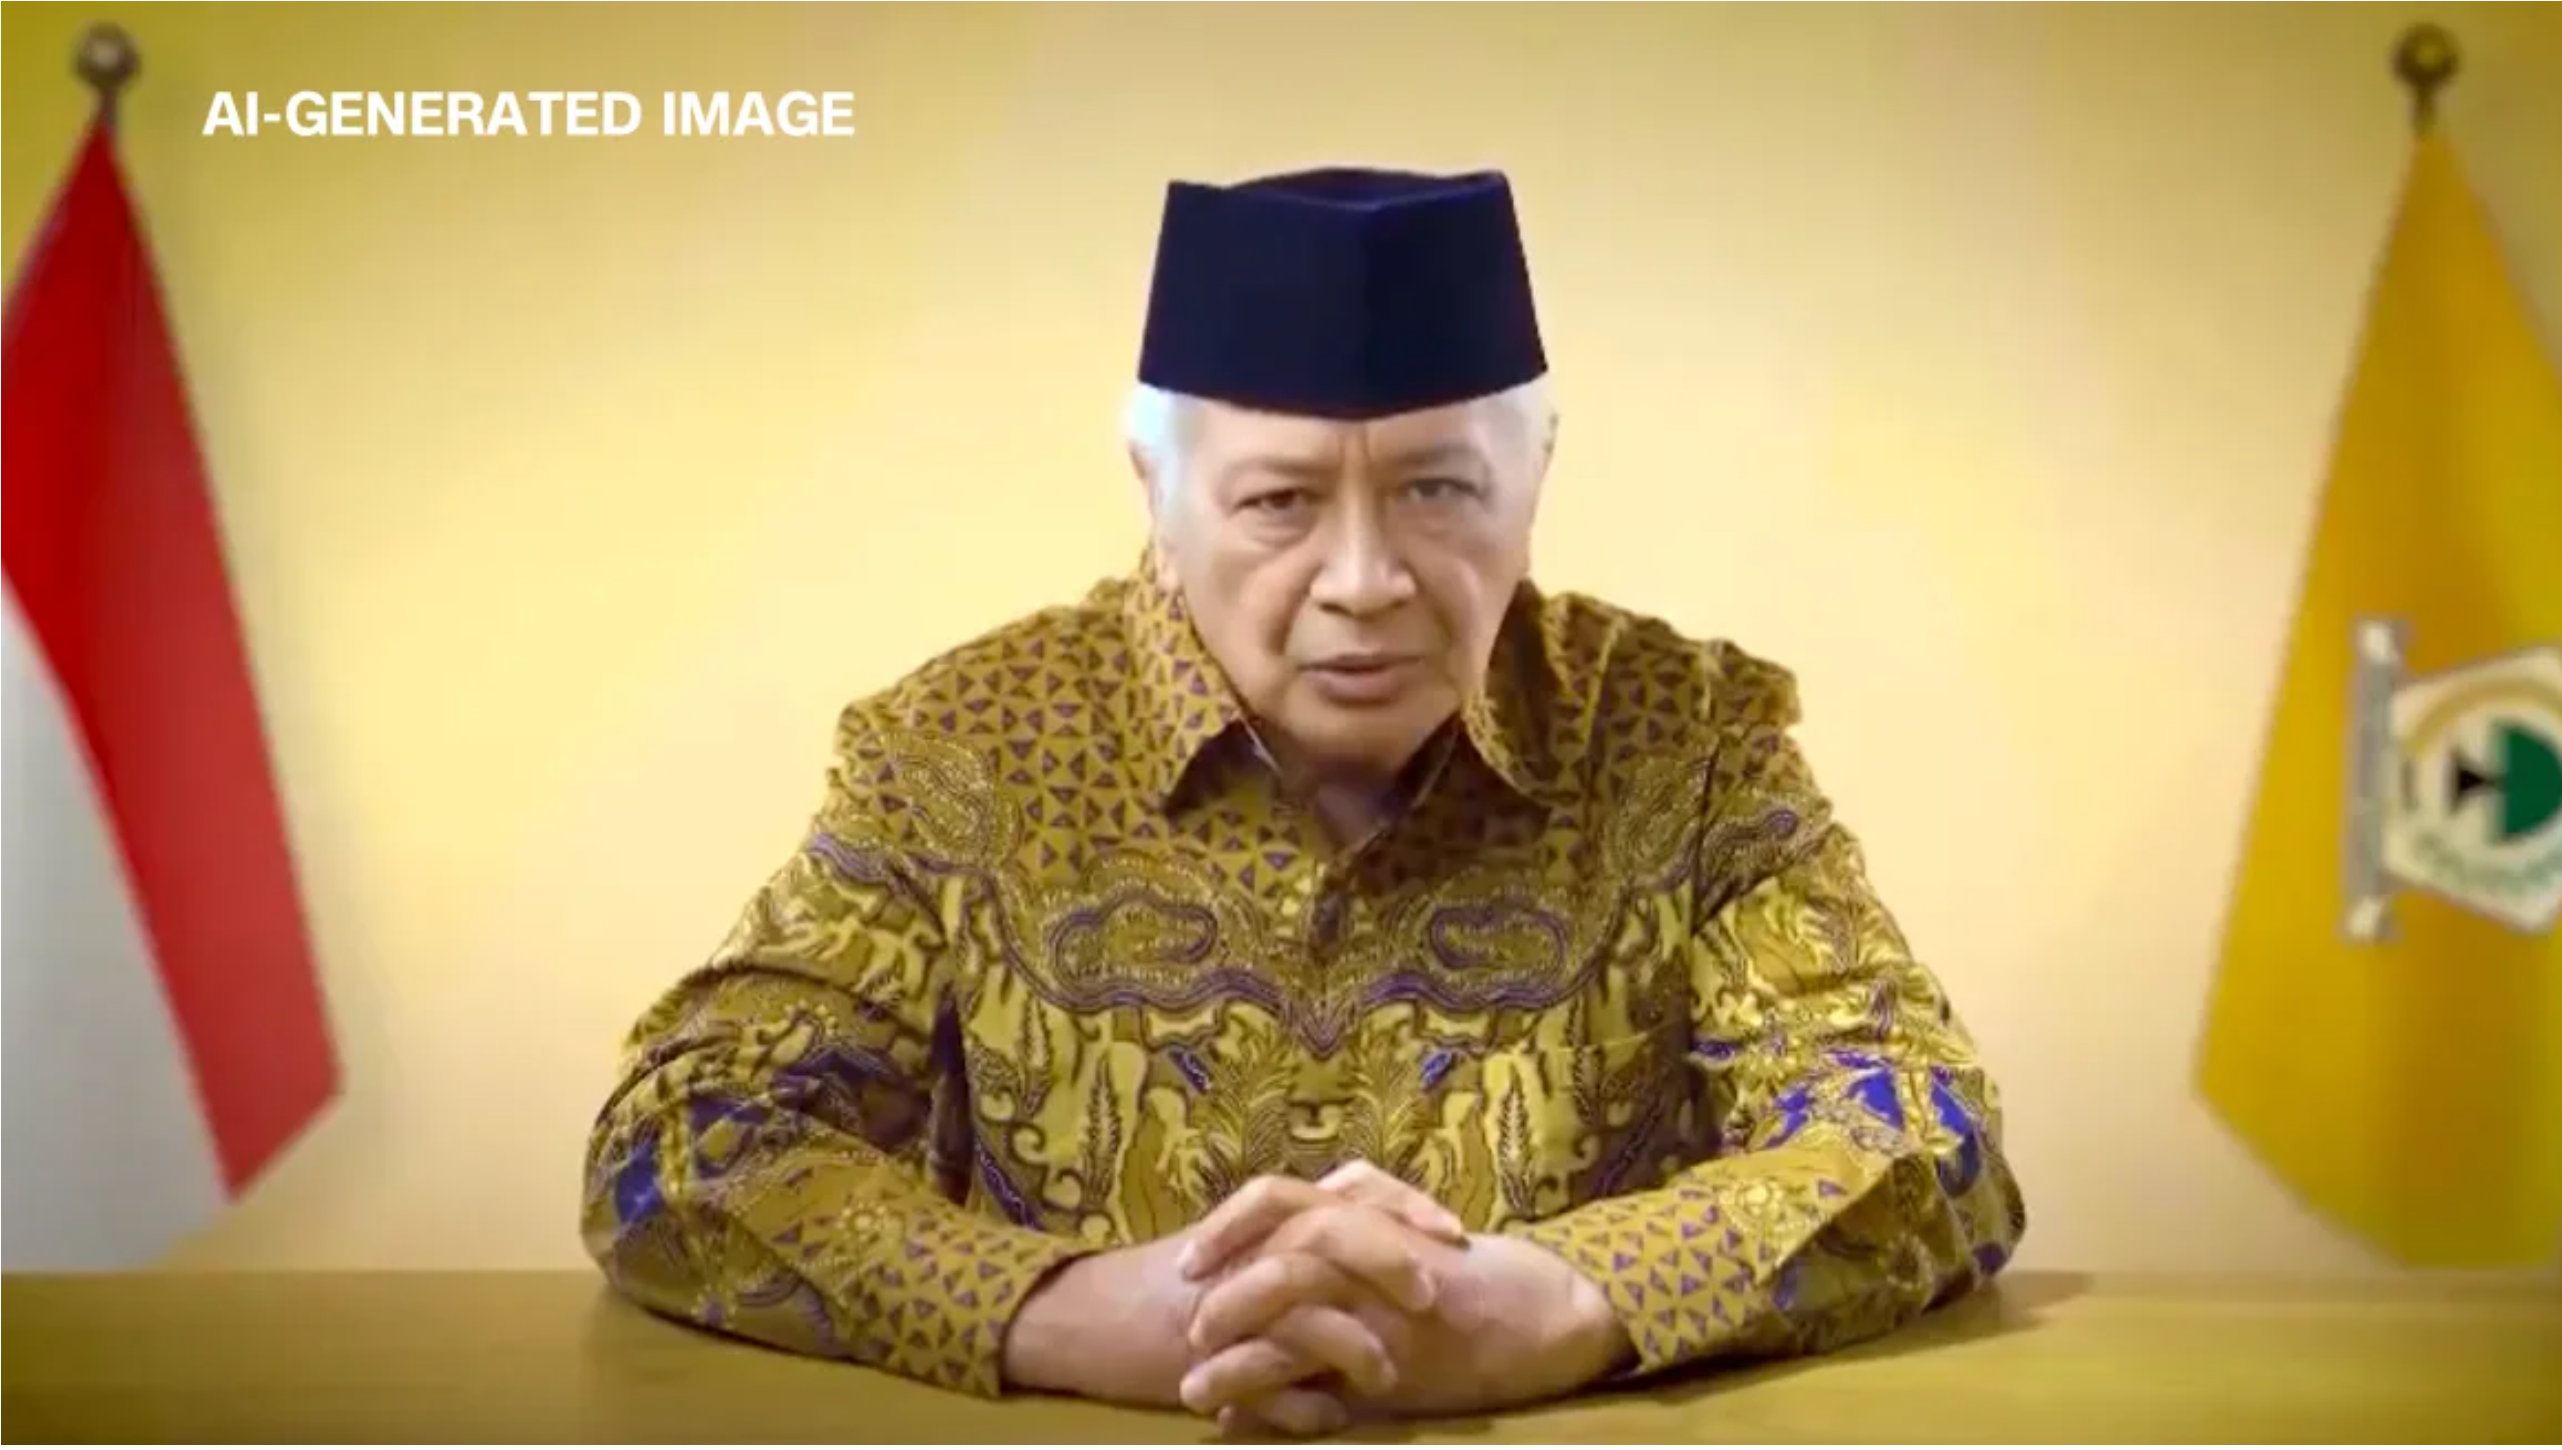
\includegraphics[width=\textwidth]{images/deepfake_suharto.png}
            \caption{Deepfake of deceased former Indonesian dictator Suharto | Erwin Aksa/X}
       
            \end{figure}
            \begin{figure}[htbp]
            \label{fig2}
            \centering
        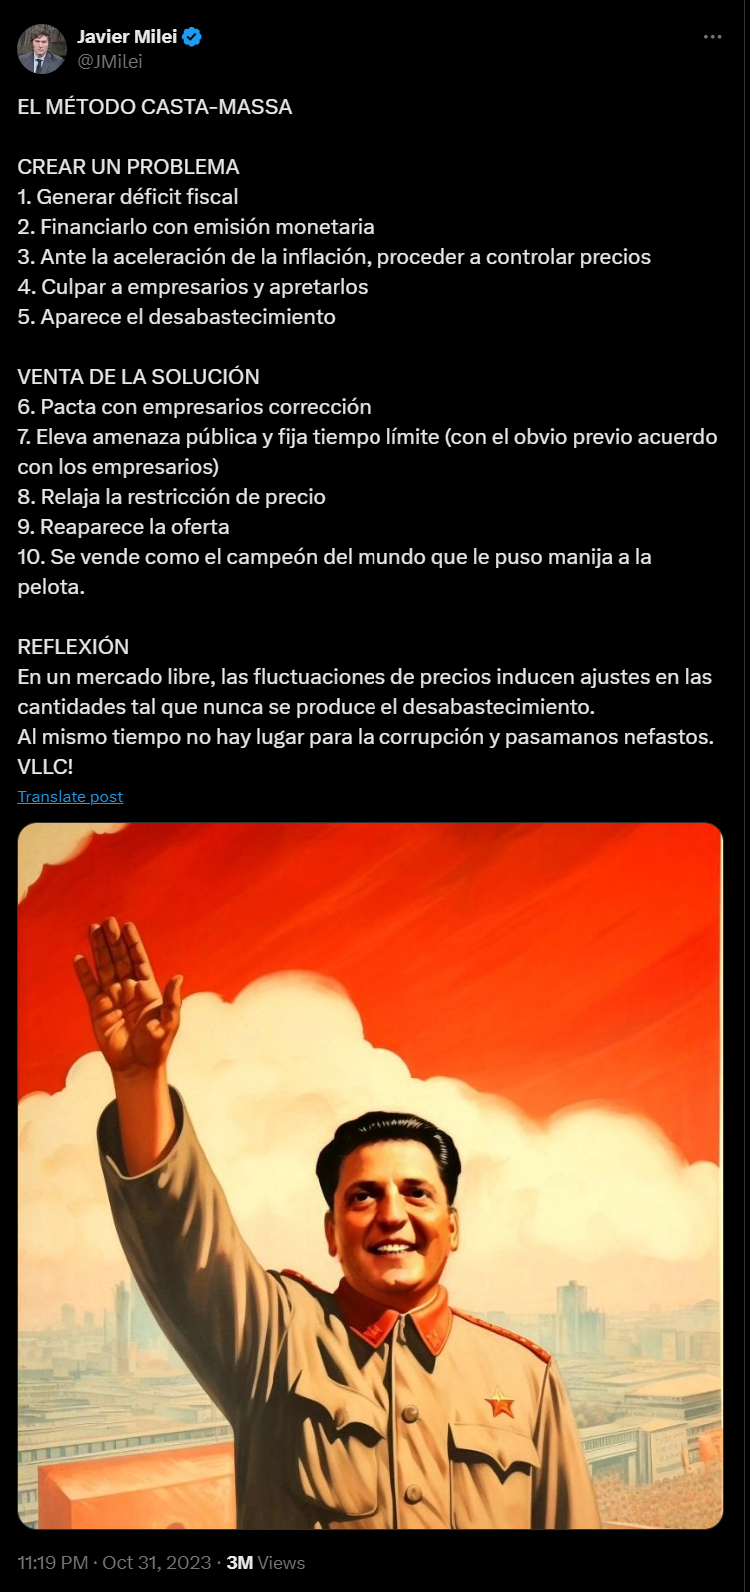
\includegraphics[width=250px]{images/gen_ai_massa_communist.png}
            \caption{AI-generated image depicting presidential candidate Massa as Chinese communist | Javier Milei/X}
        
            \end{figure}
\end{document}